\documentclass[12pt]{report}

\usepackage[english]{babel}
\usepackage[utf8x]{inputenc}
\usepackage{amsmath}
\usepackage{graphicx}
\usepackage{multirow}
\usepackage[hypcap]{caption}
\usepackage{setspace} 
\usepackage{float}

\title{Lab 6: Material Selection for Design}
\author{Zachary Tschirhart \\
	\small \\
        \small EID: zst75 \\
	\small Department of Aerospace Engineering and Engineering Mechanics \\
	\small \textbf{ASE 324L (Mon 2:00-5:00)} \\
	\small Unique: 13740}

\date{March 17, 2014}


\begin{document}
\maketitle

\setcounter{secnumdepth}{0}

\section{Introduction}
\doublespacing

In order to optimize the design of a small satellite antenna, choosing an appropriate material and size/shape of the apparatus is needed. In order to do this, a database of materials was used and certain parameters were used to whittle down the available materials. This process lead to about ten materials that had the best qualities for the intended purpose.

\section{Summary of Design Requirements and Derivation of Materials Indices}

The design requires that the boom handle a thermal gradient of 1000 BTU/hr with a minimized tip deflection. According to the standard heat conduction law below,

\begin{equation}
  \.{q} = \lambda L t \frac{\Delta T}{h}
  \label{equation:equation1}
\end{equation}

In order to keep heat flux at 1000 BTU/hr and have the most freedom with shape of the boom, a minimization of the thermal conductivity will be needed. 

The following equation can describe the relationship of the deflection of the boom.

\begin{equation}
  \delta = \frac{L^2}{2 \frac{h}{\alpha \Delta T}}
  \label{equation:equation2}
\end{equation}

In order to minimize the deflection, depth of the boom needs to be maximized while the coefficient of thermal expansion needs to be minimized. 

In addition to the thermal properties, the natural frequency of the bending mode should be maximized, which correlate to the below equation being maximized. 

\begin{equation}
  f = \frac{3.52}{2 \pi} \sqrt{\frac{EI}{\rho h t L^5}}
  \label{equation:equation3}
\end{equation}

In the equation, f needs to be maximized, so Young's Modulus and the second moment of cross-secional area of the beam needs to be maximized, while the depth, thickness, and density of the material need to be minimized.

The mass of the structure also needs to be minimized, but the above analysis already considers this.

Also to reduce interference with the electronic equipment, non-magnetic materials must be used.

Another requirement is that the antenna boom must be able to survive the shock and vibration loads during launch, so a tensile strength must be over 30 ksi and the fracture toughness needs to be greater than 10 ksi-in1/2.

The last requirement is that of cost, which is not actually a requirement but rather a desirable trait of less than $500/lbm.

The dimensions of the boom have limits as well, which are that the antenna is 10 ft in length, its tip should not deflect more than .5 inches under thermal loads, its depth is at most .5 inches, and must be no wider than 4 inches.

\section{Screening}
There was a total of four levels of stages, each whittled down the available materials by a large factor until only ten were left.

Figure one shows a graph of thermal conductivity vs. thermal expansion coefficient and filtering out the materials in the bottom left hand corner which minimize both sets. 

\begin{figure}[H]
	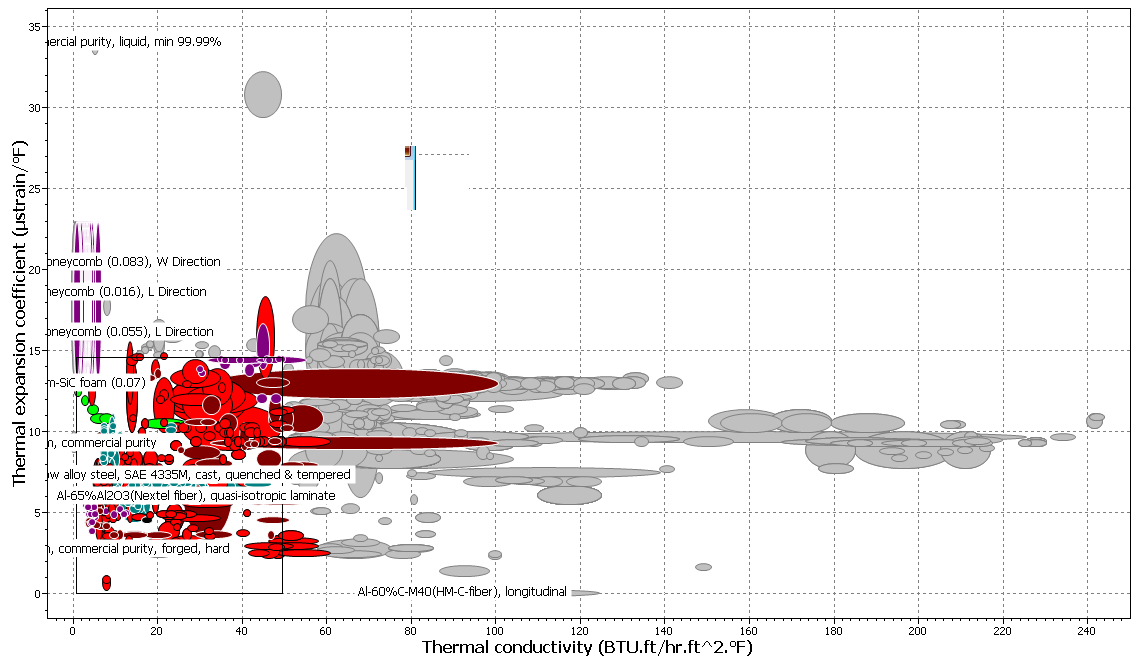
\includegraphics[width=1\textwidth]{stage1.png}
	\caption{Thermal Conductivity vs. Thermal Expansion Coefficient}
	\label{fig:Figure1}
\end{figure}


The second stage was just restricting materials to a tensile strength of at least 30 ksi, fracture toughness of 10 ksi-in1/2, and a maximum cost of $500/lbm

On the third stage, a graph of young's modulus vs. density was created while restricting materials that maximized young's modulus and minimized density.

\begin{figure}[H]
	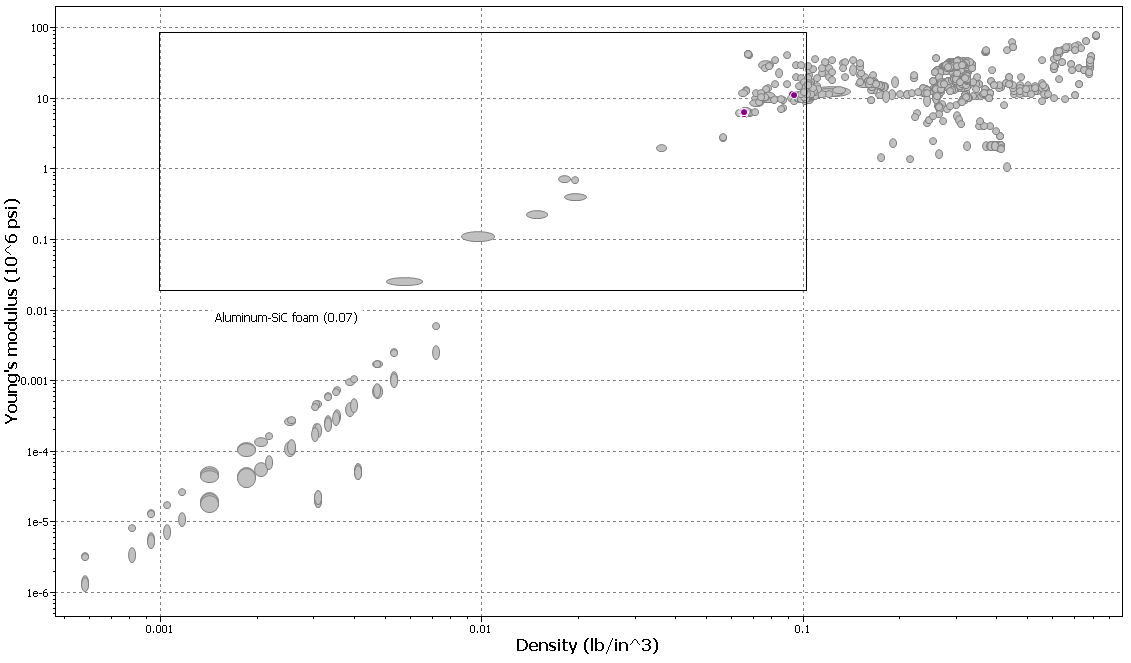
\includegraphics[width=1\textwidth]{stage3.png}
	\caption{Young's Modulus vs. Density}
	\label{fig:Figure2}
\end{figure}


On the last stage, in order to restrict materials that were not magnetic, a graph of percentage of iron vs. tensile strength was created while only choosing materials with no iron percentage and maximum tensile strength.

\begin{figure}[H]
	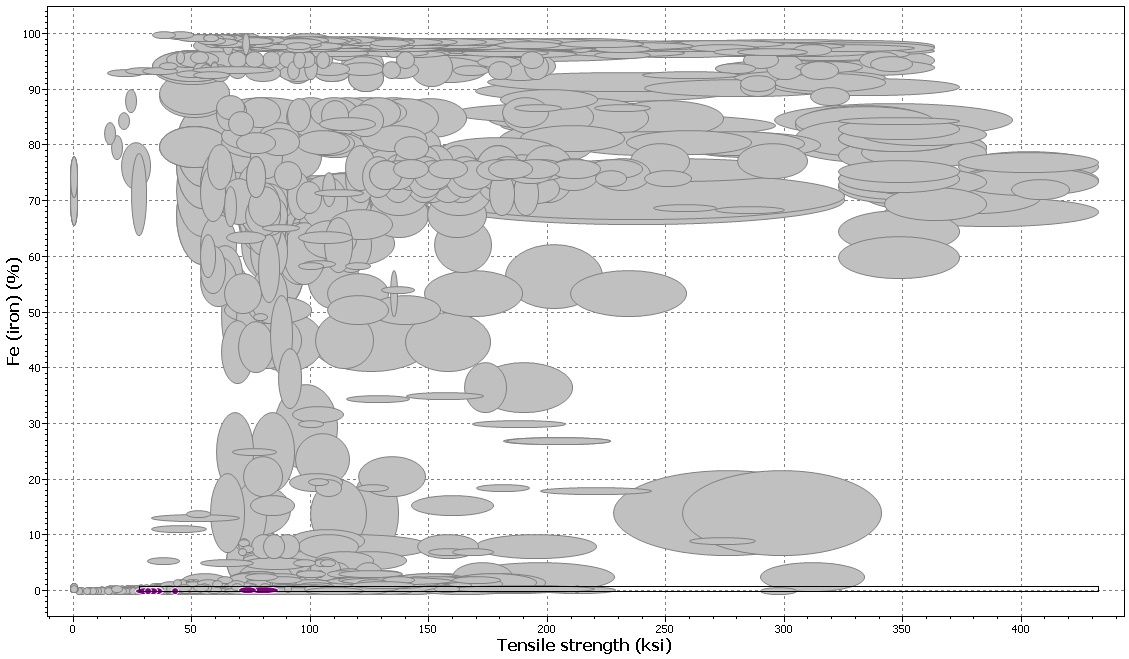
\includegraphics[width=1\textwidth]{stage4.png}
	\caption{Percentage of Fe vs. tensile strength}
	\label{fig:Figure3}
\end{figure}

\section{Ranking}
Of the materials that were left, a ranking of thermal expansion was used because of its importance in the pointing accuracy and reduced deflection. The following list is in order from best material to worst in terms of thermal expansion qualities for the purpose of using it as a boom. \\
1. Aluminum 8090, wrought, T851\\
2. Aluminum, 8091, wrought, T6\\
3. Magnesium, AM60B, cast\\
4. Magnesium, AJ62A, cast\\
5. Magnesium, AS41B, cast\\
6. Magnesium, AZ61A, cast\\
7. Magnesium, AS21B, cast\\
8. Magnesium, AE42, cast, F\\
9. Magnesium, AE44, cast, F\\
10. Magnesium, AZ80A, wrought\\

\section{Shape optimization}

After trying a combination of different shapes and sizes for the antenna boom, a hollow rectangular box will provide the best combination of positive attributes. This decision comes from maximizing the second moment of cross-sectional area of the beam, while maximizing the lowest natural frequency of the beam and deflection. The optimized depth of the beam was .25 inches and a width of 3.5 inches.


\section{Conclusion}
In conclusion the best material to use would be either the Aluminum 8090 or Aluminum 8091 because of its thermal properties, density, and cost. While the boom has a hollow rectangular cross-sectional area to meet the pointing requirements for the antenna. 


\end{document}
